\section{Entwurf}

\subsection{Technische Funktionen (und Funktionsabhängigkeiten)}

\subsubsection{Einen Account erstellen}

	\begin{figure}[H]
		\centering
		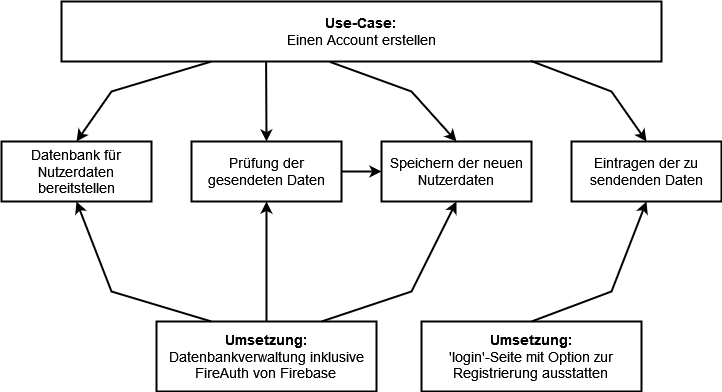
\includegraphics[width=0.5\textwidth]{img/diagrams/Anforderung-Registrieren}
	\end{figure}

\subsubsection{In Account einloggen}

	\begin{figure}[H]
		\centering
		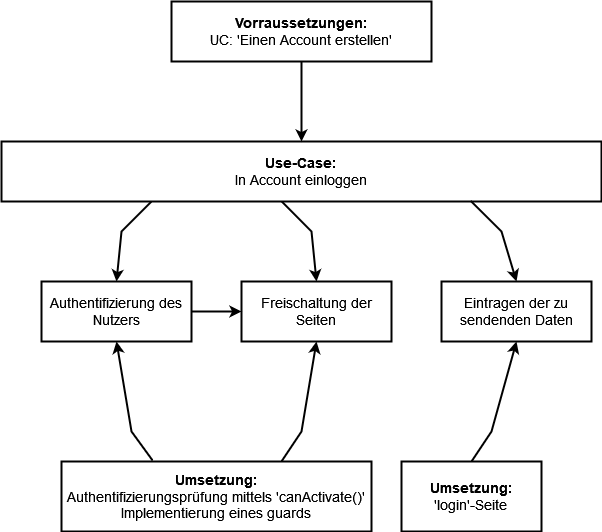
\includegraphics[width=0.5\textwidth]{img/diagrams/Anforderung-Einloggen}
	\end{figure}

\subsubsection{Eine Reise erstellen}

	\begin{figure}[H]
		\centering
		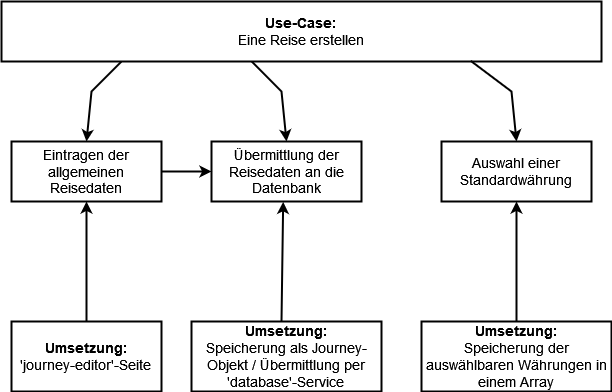
\includegraphics[width=0.5\textwidth]{img/diagrams/Anforderung-Reise_erstellen}
	\end{figure}

\subsubsection{Einer Reise beitreten}

	\begin{figure}[H]
		\centering
		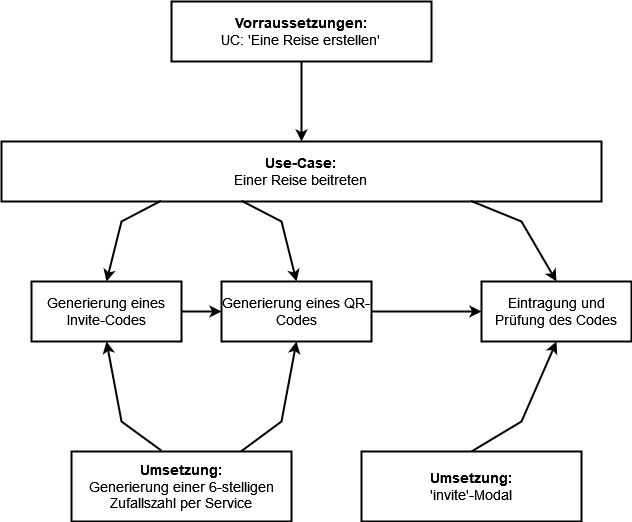
\includegraphics[width=0.5\textwidth]{img/diagrams/Anforderung-Reise_beitreten}
	\end{figure}

\subsubsection{Zahlung festhalten}

	\begin{figure}[H]
		\centering
		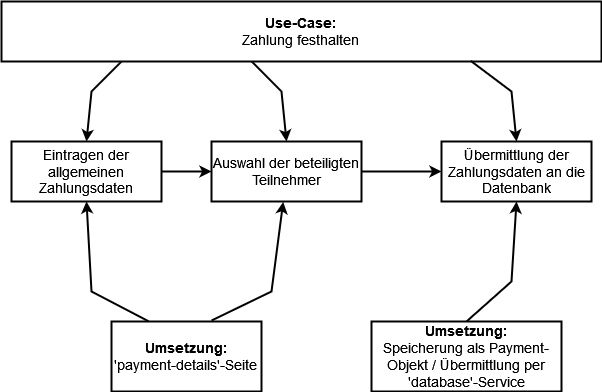
\includegraphics[width=0.5\textwidth]{img/diagrams/Anforderung-Zahlung_festhalten}
	\end{figure}

\subsubsection{Zahlung einsehen}

	\begin{figure}[H]
		\centering
		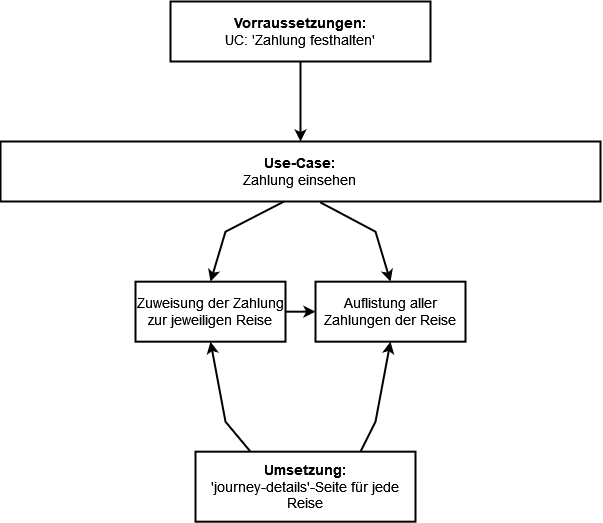
\includegraphics[width=0.5\textwidth]{img/diagrams/Anforderung-Zahlung_einsehen}
	\end{figure}

\subsubsection{Schulden einsehen}

	\begin{figure}[H]
		\centering
		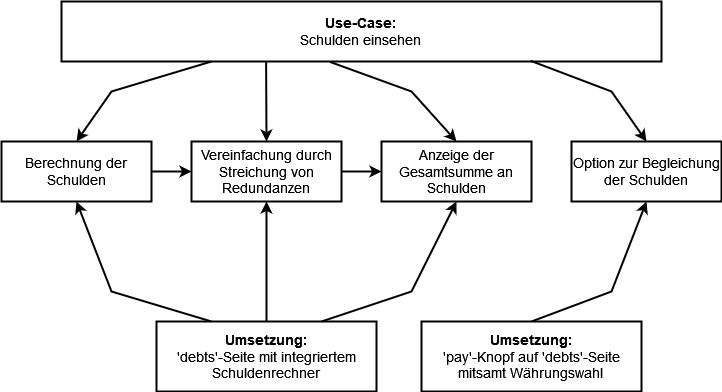
\includegraphics[width=0.5\textwidth]{img/diagrams/Anforderung-Schulden_einsehen}
	\end{figure}

\subsubsection{Reise archivieren}

	\begin{figure}[H]
		\centering
		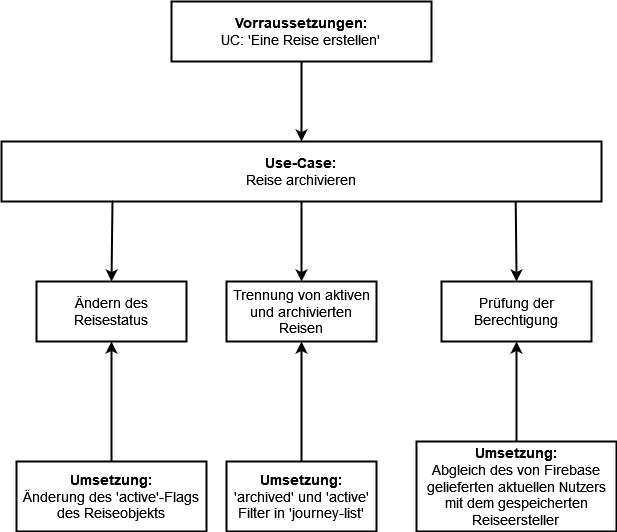
\includegraphics[width=0.5\textwidth]{img/diagrams/Anforderung-Reise_archivieren}
	\end{figure}

\subsubsection{Reisen einsehen}

	\begin{figure}[H]
		\centering
		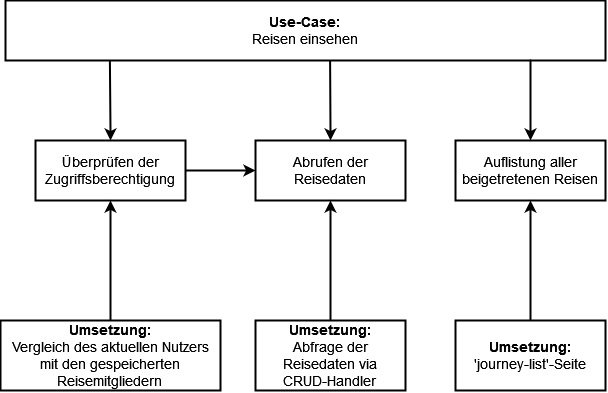
\includegraphics[width=0.5\textwidth]{img/diagrams/Anforderung-Reise_einsehen}
	\end{figure}

\newpage

\subsection{Datenmodell}

\subsubsection{Ursprüngliches Datenmodell}
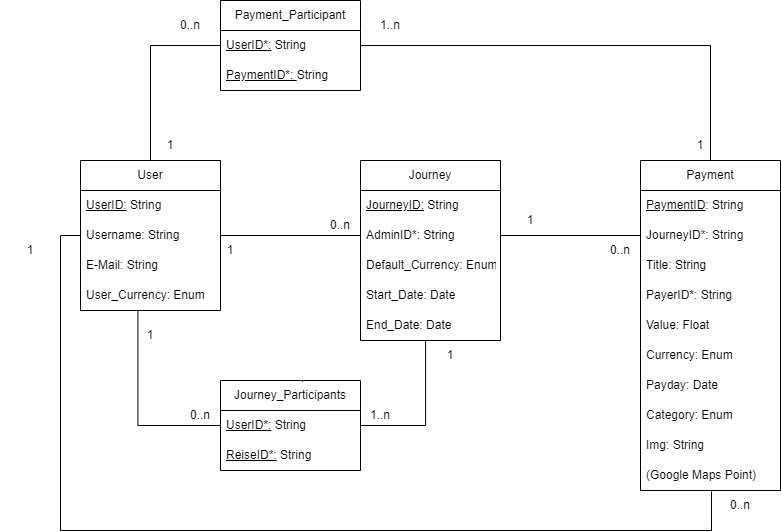
\includegraphics[width=170mm]{img/diagrams/Geplantes_UML.drawio}

\subsubsection{Finales Datenmodell}
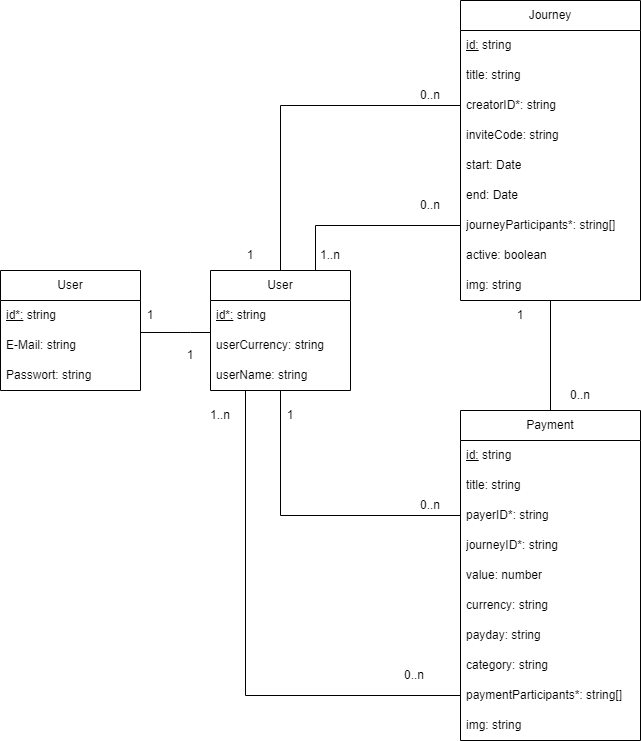
\includegraphics[width=170mm]{img/diagrams/Umgesetztes_UML.drawio}

\subsection{Strukturmodell (Aufbau)}

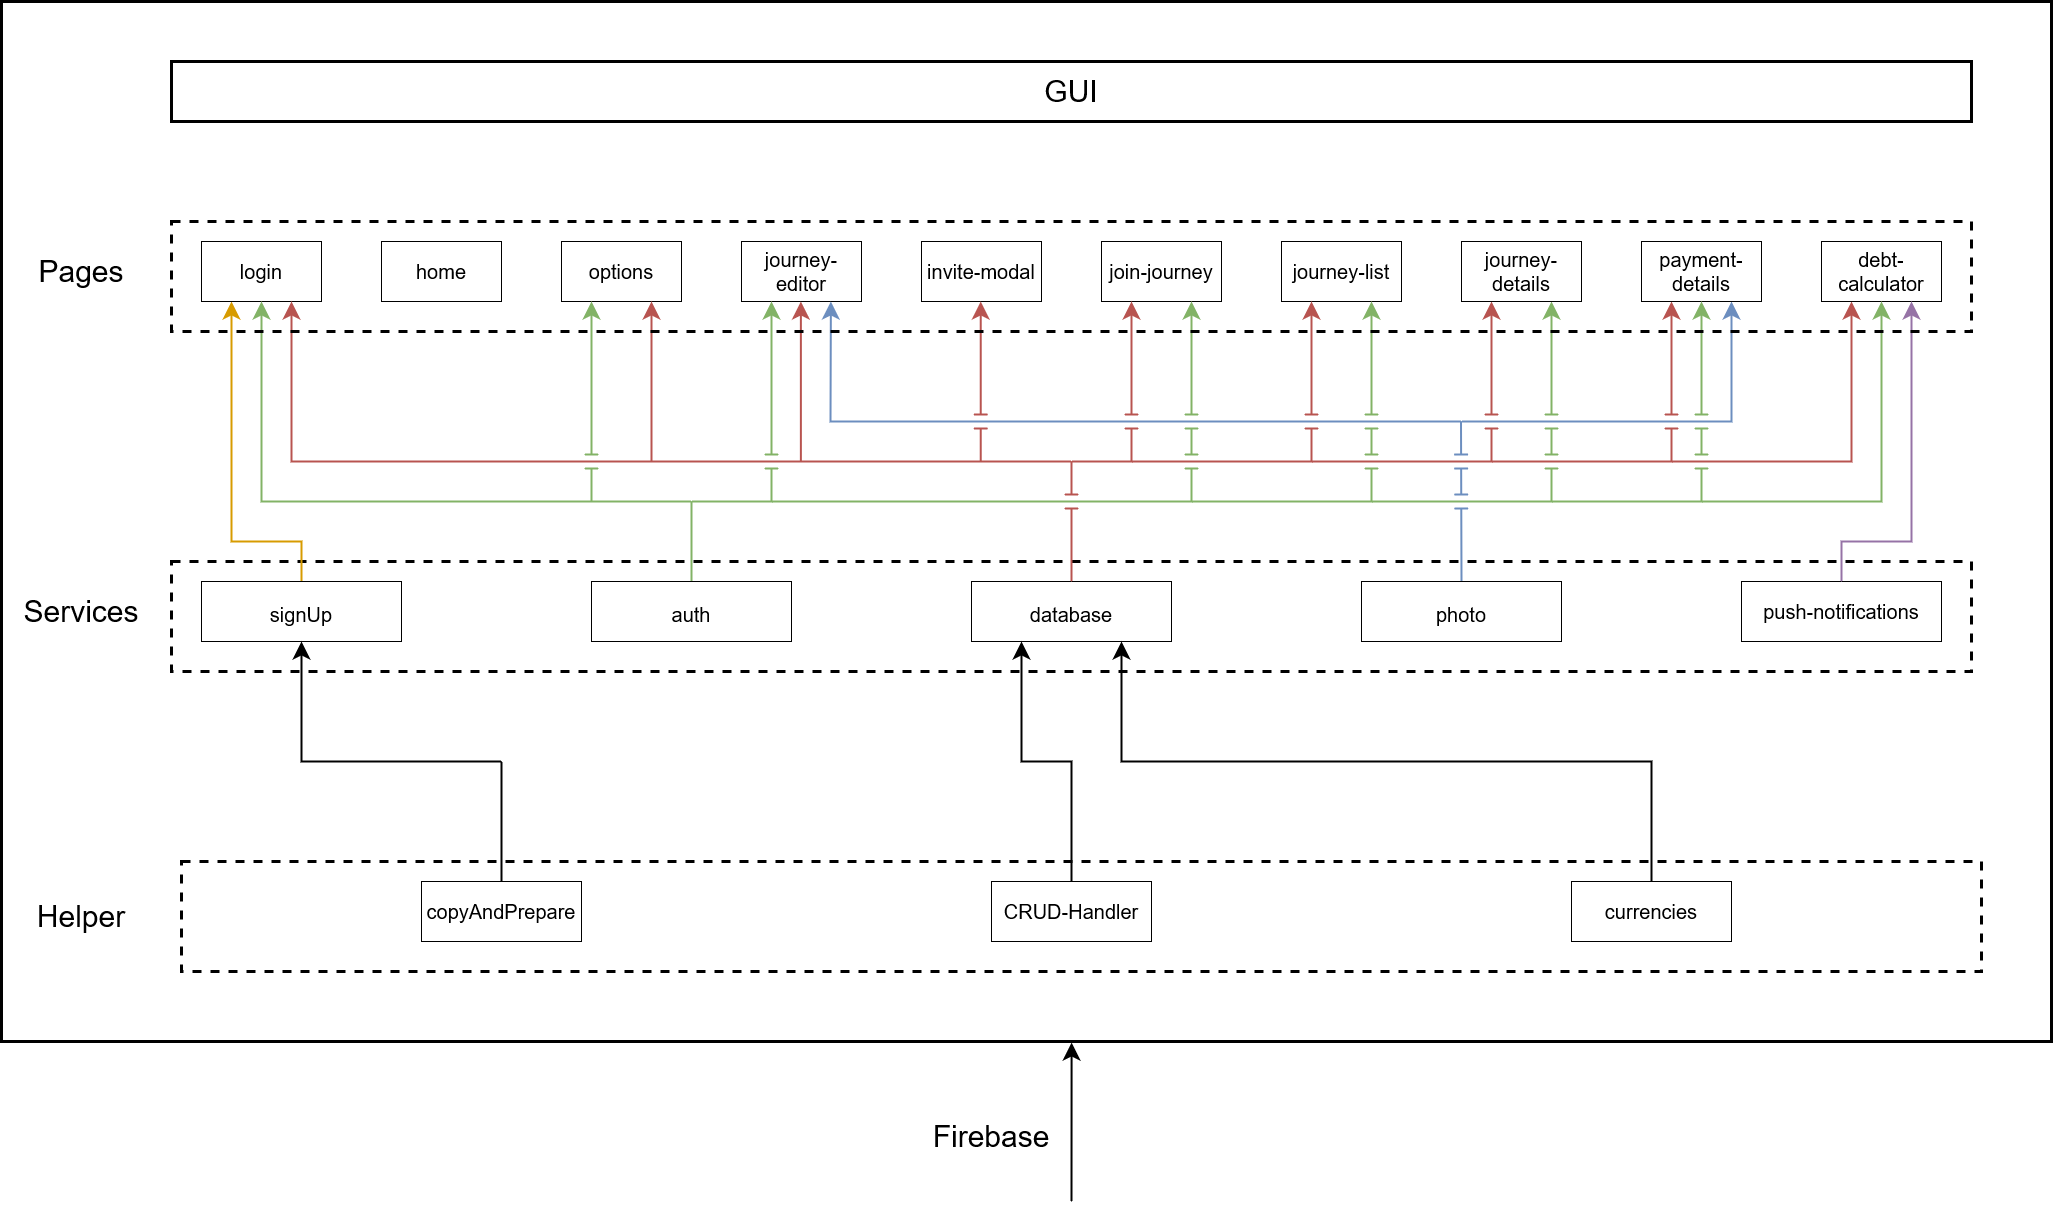
\includegraphics[width=170mm]{img/diagrams/Strukturdiagramm}

\subsection{Testfälle}

Die Auflistung der Testfälle befindet sich im Testprotokoll (Siehe Kapitel \ref{Tests}).